\documentclass[tikz]{standalone}

\begin{document}

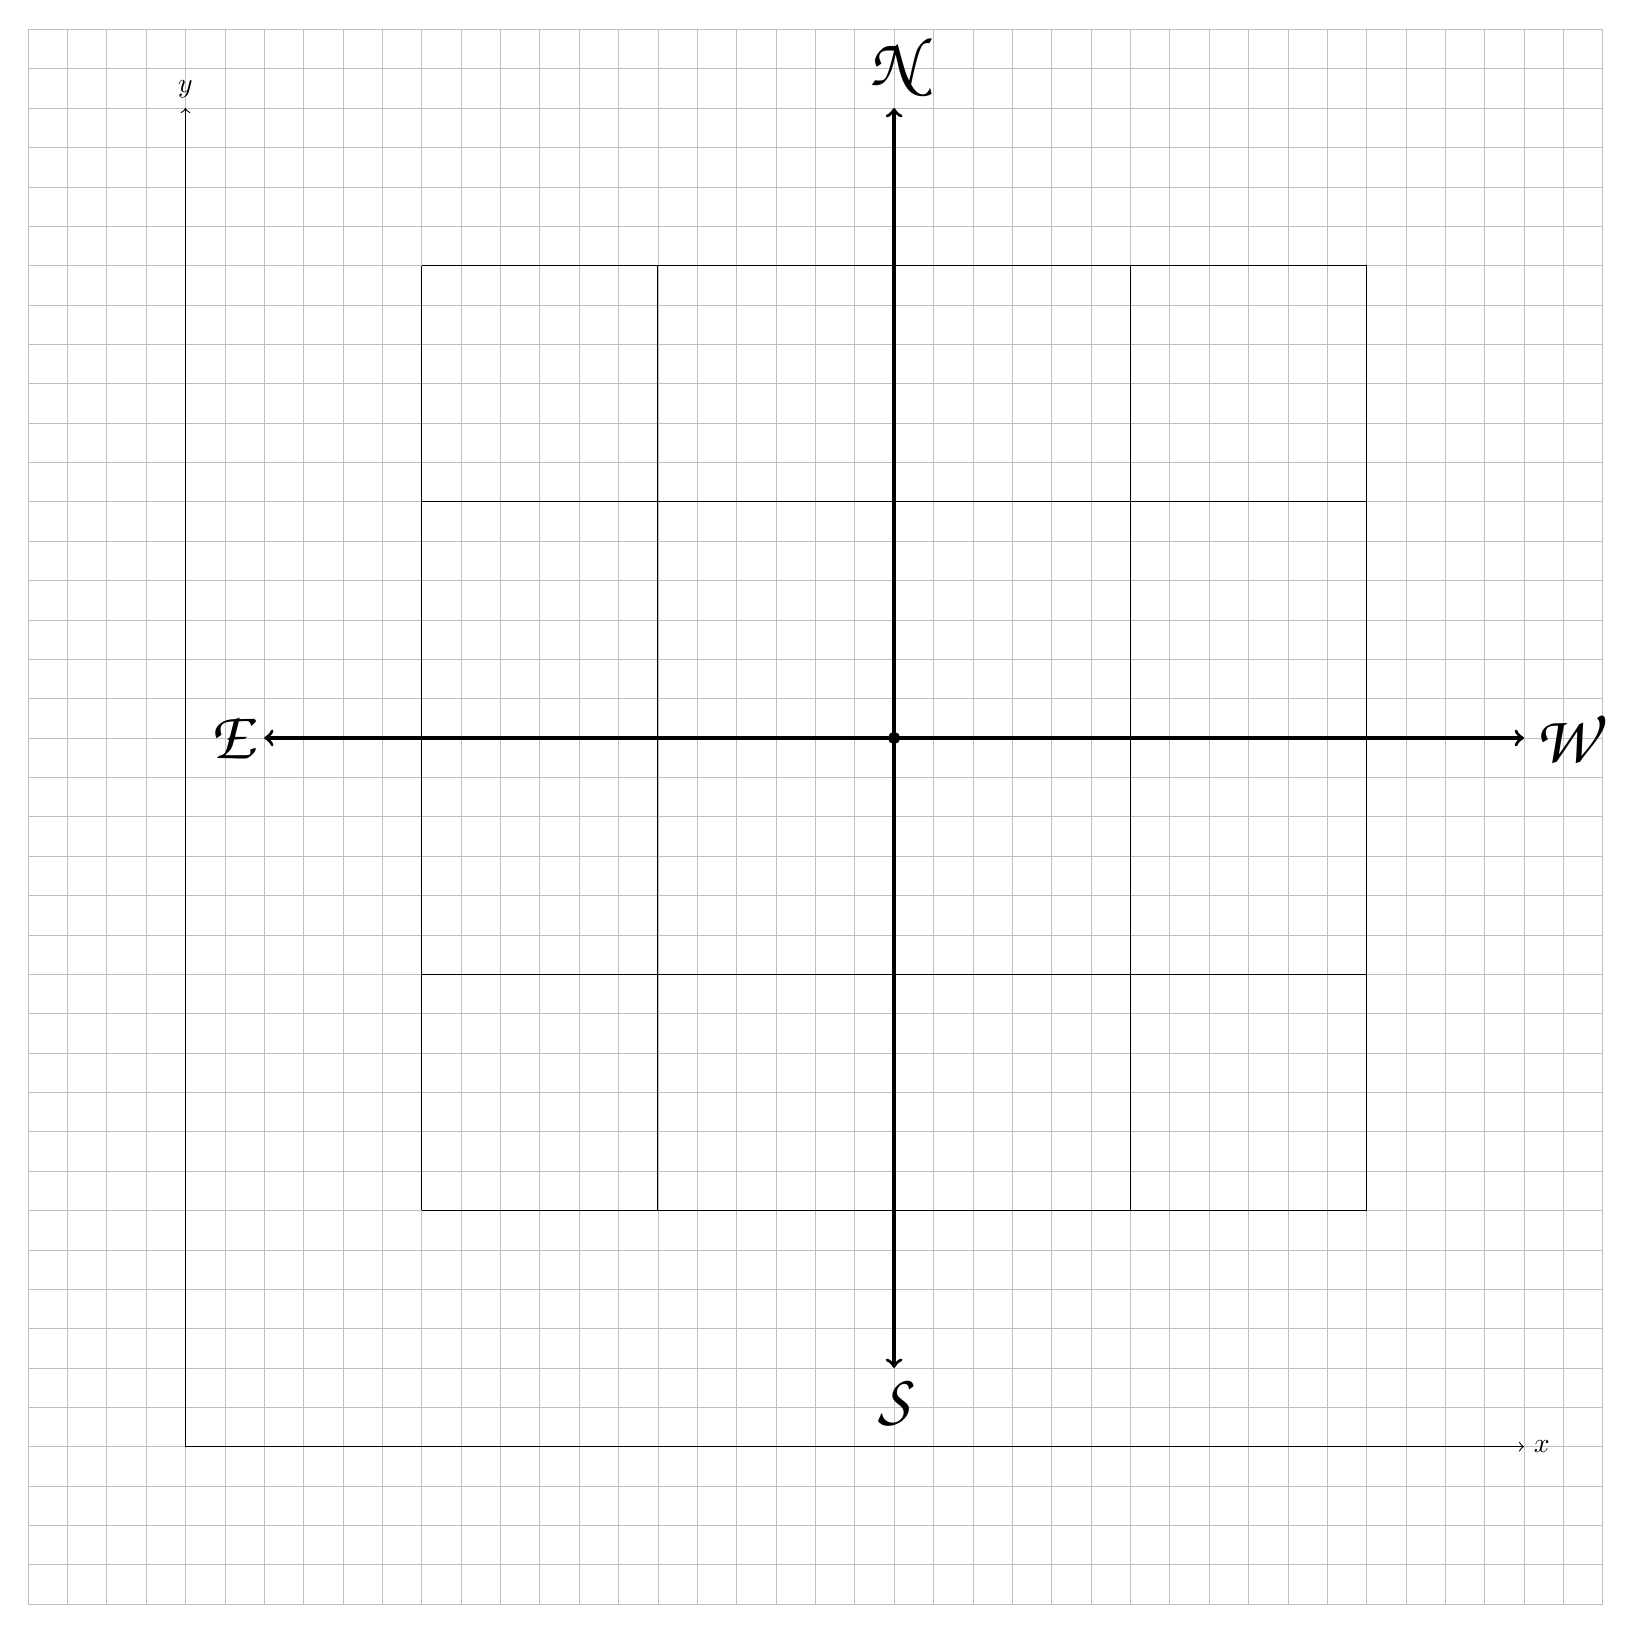
\begin{tikzpicture}
  \draw[step=0.5, lightgray, very thin] (-2,-2) grid (18,18); 
  \coordinate (y) at (0,17);
  \coordinate (x) at (17,0);
  \draw[<->] (y) node[above] {$y$} -- (0,0) -- (x) node[right] {$x$};
  \draw[step=3] (3,3) grid (15,15);

  \path 
    coordinate (center) at (9,9)
    coordinate (north)  at (9,17)
    coordinate (south)  at (9,1)
    coordinate (east)   at (1,9)
    coordinate (west)   at (17,9)
  ;

  \draw[fill] (center) circle [radius=2pt];
  \draw[->, very thick] (center) -- (north) node[above] {\Huge\fontfamily{pzc}\selectfont{}N};
  \draw[->, very thick] (center) -- (south) node[below] {\Huge\fontfamily{pzc}\selectfont{}S};
  \draw[->, very thick] (center) -- (east) node[left] {\Huge\fontfamily{pzc}\selectfont{}E};
  \draw[->, very thick] (center) -- (west) node[right] {\Huge\fontfamily{pzc}\selectfont{}W};


\end{tikzpicture}

\end{document}
